\chapter{Related work}
\label{ch:related_work}

\section{Existing frameworks for state machine applications}
State machine -based systems is a well-established concept in the world of software, and several frameworks already exist for developing applications based on this concept. These frameworks vary in implementation language, design method and portability, and some of their main properties will be outlined in this section. These frameworks will be used for comparison when evaluating Lua/eLua for state machine -based systems.

\subsection{Reactive Blocks}
Reactive Blocks (\url{http://www.bitreactive.com/})is a Java-based framework for developing state machine applications. It offers integration with the Eclipse IDE, and is essentially a code/application generator with a graphical interface, tailored for event-driven and concurrent systems. Application design is done by creating, connecting and combining various “building blocks”. These building blocks consist of three parts:
\begin{itemize}
	\item Activity diagram \ref{state_machine_systems}: describes the internal behavior and logic of the block.
	\item External state machine: serves as an interface towards other blocks and the enclosing application. Defines which input signals are allowed in a given state, transitions associated with an input signal and a state, and any output signals resulting from the transition.
	\item Java methods that handle any operations performed as part of a transition.
\end{itemize}

An example of a building block in Reactive Blocks is displayed in figure \ref{figure:reactive_blocks}.

\begin{figure}[h]
	\centering
	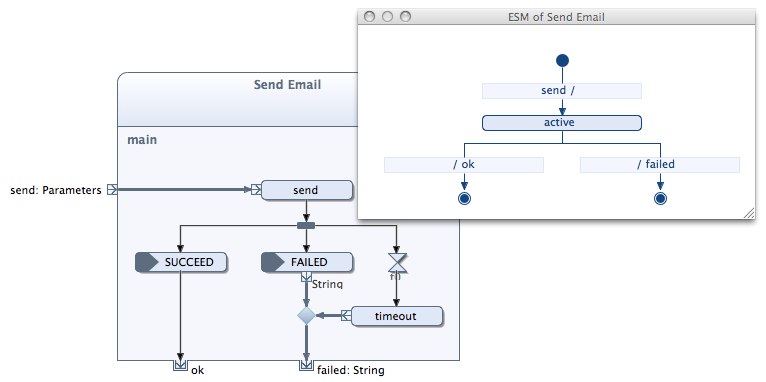
\includegraphics[scale=0.5]{img/reactive_blocks.png}
	\caption[A building block in Reactive Blocks]{An example of a building block in Reactive Blocks, displaying the activity diagram (to the left) and the external state machine (to the right). Image source: \url{http://reference.bitreactive.com/doc/building_blocks} \label{figure:reactive_blocks} }
\end{figure}

The Reactive Blocks SDK has various advantages for development of state machine -based applications:
\begin{itemize}
	\item It comes with a built-in verification tool that helps the user discover and handle logical mistakes and design flaws in the application. The framework also integrates with JUnit, for testing separate components and operations.
	\item Instead of a large and complex code base, the application consists of a hierarchy of connected building blocks, with functionality and logic defined at the design level. This generally makes projects easier to organize, maintain and extend.
	\item With the built-in runtime support system and implementation at the design level, concepts like forking, waiting and synchronization are simple, making creation of concurrent systems almost a triviality.
	\item Java has a huge base of libraries that may be combined with Reactive Blocks to provide functionality and application development on higher levels.
\end{itemize}

However, one fundamental disadvantage is that any applications created with Reactive Blocks require a Java VM. This creates an obstacle when working on embedded systems, because the Java SE Embedded VM currently only supports the \textit{most powerful} embedded systems \cite{website:java_embedded_vm}. Memory requirements range from 130KB RAM/350KB ROM (minimal configuration) to several MB for both RAM and ROM (full configuration), which is more than what you can expect to find in a typical light

\subsection{RKH}
RKH (\url{http://rkh-reactivesys.sourceforge.net}) is a C-based development tool for implementing state machine -based systems. It is specifically designed to work on embedded systems, and consists of various platform-independent modules. The software provides a cooperative scheduler, timer and event managers, as well as a graphical interface to help designing state machines based on UML state tables. Like Reactive Blocks, RKH generates and compiles code that can be run directly. An example of a transition table statement in RKH is displayed in figure \ref{figure:rkh_transition}.

\begin{figure}[h]
	\centering
	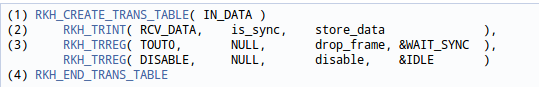
\includegraphics[scale=0.7]{img/rkh_transition_table.png}
	\caption[A transition table statement in RKH]{An example of a transition table statement in RKH, written in C code. Each line in the statement defines a transition with input signal, guard function, action function and target state. Image source: \url{http://rkh-reactivesys.sourceforge.net/qref.html} \label{figure:rkh_transition} }
\end{figure}


RKH has some particularly strong advantages when developing state machine -based applications on embedded systems:
\begin{itemize}
\item RKH is fairly platform-independent, and already built to support many platforms and processors (linux, RTOS, mbed etc…). Additionally, the modules are customizable and the project is open source, meaning it can be adapted also to custom platforms.
\item The system has a very small memory footprint, making it usable also for minimal embedded systems.
\item Application design with state tables and diagrams is simple and maintainable.
\end{itemize}

However, for the less experienced programmer, RKH also provides some challenges:
\begin{itemize}
	\item While parts of the RKH interface can be intuitively understood, other parts (like declaring actions) require at least basic knowledge of C programming. Programming in C is considered complex and difficult compared to “higher level”-languages like Java, Python or Lua.
	\item Customization and adaptation of the software platform requires knowledge of and skills in C programming.
	\item External libraries implementing functionality are fairly limited in C, and must in some cases be adapted to the relevant platform anyway. This means C programming and extra work is required for anything but standard state machine functionality.
\end{itemize}

\subsection{Quantum Leaps}
http://www.state-machine.com/qm/index.php

\subsection{IntelliWizard}
http://www.codeproject.com/Articles/10801/Design-State-Machine-Engine-for-embedded-system-de

\section{Lua and embedded systems}

\subsection{Mihini}

\subsection{LEGO Mindstorms}
\cite{chapter:porting_lua_microcontroller}

\subsection{Einsatz von Lua in Embedded Systems}
http://www.amazon.de/Lua-Einsatz-von-Embedded-Systems/dp/3907857151/

\begin{itemize}
	\item DLL <-> Lua interface
	\item Lua on embedded DOS system
	\item Lua on embedded Linux system
	\item Lua on FOX Board G20
	\item eLua on mbed
	\item Peripherals and I/O
	\item Benchmarks and performance measurements
	\item SWIG: http://en.wikipedia.org/wiki/SWIG
	\item toLua: http://www.tecgraf.puc-rio.br/~celes/tolua/
	\item examples: http://sourceforge.net/projects/lua/
\end{itemize}